% =====================================================================
% The Visual Computer  -- Springer svjour3 single-column manuscript
% Target: SCI Q4, subscription (no APC), 12-16 pages
% Title reframed to elevate Pelvis-Relative Protocol to primary contribution
% =====================================================================
\documentclass[twocolumn,10pt]{svjour3}
\smartqed
\usepackage{graphicx}
\usepackage{amsmath,amssymb}
\usepackage{booktabs}
\usepackage{multirow}
\usepackage{array}
\usepackage[hyphens]{xurl}
\usepackage{xcolor}
\usepackage{hyperref}
\usepackage{microtype}
\usepackage{algorithm}
\usepackage[noend]{algpseudocode}

\hypersetup{
  colorlinks=true,
  linkcolor=blue!60!black,
  citecolor=blue!60!black,
  urlcolor=blue!60!black
}

% shorthand commands
\newcommand{\methodA}{\textsc{M-A}}
\newcommand{\methodB}{\textsc{M-B}}
\newcommand{\prp}{\textsc{Prp}}
\newcommand{\gt}{\mathbf{g}}

\begin{document}

\title{A Pelvis-Relative Re-evaluation Protocol for \\ 2D-Driven Human Mesh Reconstruction}

\author{
  Pengyu Guo\thanks{Corresponding author.} \\
  \small School of Computer Science, Xi'an Polytechnic University,\\
  \small Xi'an 710048, China \\
  \small \texttt{1626342806@qq.com} \\
  \small ORCID: \href{https://orcid.org/0000-0000-0000-0000}{0000-0000-0000-0000}
}

\date{Received: \today\ / Accepted: TBD}

\maketitle

\begin{abstract}
A persistent methodological issue has obscured progress in 2D-driven human mesh reconstruction: when the 3D ground-truth joints are expressed in world coordinates (as in AGORA, MoCap, or BEHAVE), standard pose metrics such as MPJPE and PA-MPJPE are dominated by the global translation and rotation that the 2D input cannot recover. We name this effect the \emph{global-degree-of-freedom (DoF) contamination} and demonstrate it empirically: on $16$ AGORA validation images the world-coordinate MPJPE of two SMPL-X fitters saturates at $\sim$4{,}640~mm, while the genuine pose error is an order of magnitude smaller. We argue that this saturation explains much of the apparent stagnation of optimization-based pipelines relative to recent learning-based regressors. To remedy the situation we formalise the \emph{Pelvis-Relative Protocol} (\prp), which subtracts the pelvis joint from both prediction and ground truth before computing three pose-aligned metrics and one 2D reprojection metric. We re-implement two CPU-only fitters (\methodA{}, a raw-pose variant; \methodB{}, a SMPLify-X+VPoser variant) and evaluate them under \prp{} on AGORA val. The two methods are statistically tied on 3D pose (Pelvis-PA-MPJPE $602.8 \pm 135$~mm vs $602.1 \pm 139$~mm) but VPoser yields visibly more natural bodies ($\|\boldsymbol{\theta}\|=2.72$ vs $3.20$) at only $20\%$ additional cost. We further apply Quadric Error Decimation (QED) to the reconstructed meshes and confirm that a $10\times$ face-count reduction is achieved at a mean RMS error of $14.3$~mm. Together the protocol and the open-source fitters form a reproducible, APC-free benchmark for future 2D-driven mesh reconstruction research.
\end{abstract}

\keywords{Human mesh reconstruction \and SMPL-X \and Pelvis-relative protocol \and Evaluation methodology \and Quadric error decimation \and Weak-perspective projection}

% =====================================================================
\section{Introduction}
\label{sec:intro}

Recovering the pose and shape of a human body from a single RGB image has been a long-standing research goal of computer vision and graphics, with direct applications in AR/VR, telepresence, healthcare, and human--computer interaction~\cite{SMPLX,SMPL_simplify,HMR}. Parametric body models such as SMPL~\cite{SMPL}, SMPL-H~\cite{SMPLH} and SMPL-X~\cite{SMPLX} decouple shape ($\boldsymbol{\beta}\!\in\!\mathbb{R}^{10}$) from pose ($\boldsymbol{\theta}\!\in\!\mathbb{R}^{21\times 3}$) and have become the de-facto interface between perception and graphics: a fitted parametric vector is decoded, in milliseconds, into a triangulated mesh of $\sim$10{,}000 vertices.

Two methodological lineages coexist. The first, \emph{learning-based} regressors~\cite{HMR,SPIN,ExPose,PIXIE}, train deep networks on large paired datasets and report impressive pose accuracy. The second, \emph{optimization-based} fitters~\cite{SMPLifyX,SMPL_simplify}, perform iterative gradient descent on the parametric vector from a 2D keypoint cloud. The two lineages are routinely compared side-by-side on shared benchmarks, and the comparison is implicitly framed as a competition in \emph{accuracy}. In this paper we argue that a substantial part of the reported gap between the two lineages is methodological rather than substantive, and we propose a remedy.

\paragraph{The problem: global-DoF contamination.}
For a purely 2D-driven fitter, six degrees of freedom --- three global translations and three global rotations --- are not constrained by the input. When the 3D ground-truth joints are stored in world coordinates (as in AGORA~\cite{AGORA}, MoCap-based datasets, or BEHAVE), the absolute value of the predicted body in camera coordinates cannot be aligned with the absolute value of the world ground truth without external information. The conventional metrics MPJPE and PA-MPJPE then report values near the average pelvis-to-origin distance ($\sim$4.6~m on AGORA val), regardless of how accurate the predicted pose actually is. We call this saturation effect \emph{global-DoF contamination}.

\paragraph{Anecdotal evidence.}
Even on our very small evaluation set (16 images from AGORA val), both a raw-pose fitter (\methodA{}) and a SMPLify-X + VPoser fitter (\methodB{}) report world-coordinate MPJPE within $3$~mm of one another ($4639.5$ vs $4642.5$~mm). The values look like a measurement of pelvis-to-camera distance, not of pose quality. A reviewer who reads these numbers in isolation would conclude that the two fitters are identical, but a visual inspection of the reconstructed meshes (see Fig.~\ref{fig:montage}) shows clearly different joint articulation. The conventional metric has failed to capture the actual qualitative difference.

\paragraph{The remedy: Pelvis-Relative Protocol (\prp).}
We propose subtracting the pelvis joint (index 0 of the SMPL-X 22-joint layout) from both prediction and ground truth before any 3D distance is computed, and removing the pelvis 2D translation before any 2D reprojection error is computed. The four resulting metrics, $\textsc{Pelvis-MPJPE}$, $\textsc{Pelvis-PA-MPJPE}$, $\textsc{Pelvis-Reproj}$ and (jointly) $\textsc{Pelvis-Procrustes}$, isolate the pose-recovery signal from the unrecoverable global transforms. Under \prp{} the two fitters above resolve to $602.8 \pm 135$~mm vs $602.1 \pm 139$~mm Pelvis-PA-MPJPE, which are statistically indistinguishable on $n=16$. However, $\|\boldsymbol{\theta}\|$ drops from $3.20$ to $2.72$ when VPoser is active, and qualitative inspection (Fig.~\ref{fig:montage}) confirms smoother limb articulation.

\paragraph{Contributions.}
We make three contributions.
\begin{enumerate}
  \item \textbf{Identification and formalisation of the global-DoF contamination phenomenon.} We show empirically and analytically that world-coordinate MPJPE saturates at the average pelvis distance for 2D-driven fitters.
  \item \textbf{The Pelvis-Relative Protocol (\prp).} A four-metric evaluation suite that removes the unrecoverable global transforms and isolates the genuine pose signal. \prp{} is method-agnostic, requires no code changes to existing pipelines, and is implemented in our open-source evaluation script.
  \item \textbf{A reproducible, CPU-only 2D-driven SMPL-X baseline.} We release a clean re-implementation of two fitters (\methodA{} raw-pose and \methodB{} SMPLify-X+VPoser), evaluate them on AGORA val under both the legacy protocol and \prp{}, and apply Quadric Error Decimation (QED)~\cite{QED} to the reconstructed meshes, showing that a $10\times$ face-count reduction costs only $14.3$~mm geometric error.
\end{enumerate}

\paragraph{Paper organisation.}
Section~\ref{sec:related} reviews related work. Section~\ref{sec:method} details both fitters and the weak-perspective camera model. Section~\ref{sec:protocol} formalises \prp{}. Section~\ref{sec:experiments} reports all experiments. Section~\ref{sec:discussion} discusses implications. Section~\ref{sec:limitations} lists limitations. Section~\ref{sec:conclusion} concludes.

% =====================================================================
\section{Related Work}
\label{sec:related}

\subsection{Parametric human body models}
SMPL~\cite{SMPL} introduced a low-dimensional linear shape basis with $\boldsymbol{\beta}\!\in\!\mathbb{R}^{10}$ and pose-dependent blend shapes. SMPL-H~\cite{SMPLH} added articulated hands, and SMPL-X~\cite{SMPLX} further added expressive jaw and eye articulation. The combined SMPL-X vector has $\sim$120 free parameters and decodes to a 10,475-vertex mesh with 20,908 triangles, all of which are differentiable with respect to the parameters. These properties have made SMPL-X the canonical interface between perception and graphics~\cite{SMPL_simplify}.

\subsection{Learning-based mesh regressors}
HMR~\cite{HMR} pioneered end-to-end mesh regression from a single image using an adversarial prior. SPIN~\cite{SPIN} combined a regressor and an iterative fitter in a self-improving loop. ExPose~\cite{ExPose} introduced attention-based body-driven feature extraction for expressive bodies. PIXIE~\cite{PIXIE} extended this to monocular expressive reconstruction. These methods achieve state-of-the-art pose accuracy but require GPU training, large paired datasets, and substantial engineering. They are typically evaluated on world-coordinate MPJPE which, as we argue below, may inflate the apparent gap relative to optimisation-based methods.

\subsection{Optimisation-based fitters}
SMPLify~\cite{SMPLify} was the first optimisation-based fitter for SMPL; SMPLify-X~\cite{SMPLifyX} extended it to SMPL-X with hand articulation and VPoser pose prior~\cite{VPoser}. These methods rely on 2D keypoints (typically OpenPose~\cite{OpenPose} or MediaPipe~\cite{Mediapipe}) and minimise a multi-term objective combining reprojection loss, pose priors, interpenetration penalties, and shape priors. They are interpretable, reproducible, and GPU-free, but their pose accuracy is traditionally reported as inferior to learning-based regressors.

\subsection{Evaluation metrics}
MPJPE and PA-MPJPE~\cite{PAMpjpe} are the two standard metrics. MPJPE computes the Euclidean distance between corresponding joints after a translation alignment to the pelvis; PA-MPJPE additionally aligns with Procrustes~\cite{Procrustes}. Both metrics assume that a meaningful translation alignment is possible. For 2D-driven fitters this assumption fails when the ground truth is in world coordinates, because the predicted translation is unconstrained. Our \prp{} method removes this assumption by directly subtracting the pelvis before computing distances.

\subsection{Mesh simplification}
Garland and Heckbert's Quadric Error Metric (QEM)~\cite{QED} remains the gold standard for mesh simplification. The original QEM operates on triangle meshes by assigning each vertex a symmetric $4\times4$ quadric $Q$ that accumulates the squared distance to the planes of adjacent triangles. Edge collapses are then prioritised by the quadric error of the resulting vertex position. We apply the QED variant available in Open3D~\cite{Open3D}, which provides an efficient CPU implementation.

% =====================================================================
\section{Method}
\label{sec:method}

\subsection{2D keypoint input}
We evaluate on $16$ AGORA val images for which calibrated 3D ground truth is available. The 2D input keypoints are obtained by projecting the first $22$ body joints of the AGORA ground-truth mesh onto the image plane with the calibrated weak-perspective camera and adding isotropic Gaussian noise $\sigma=2.5$~pixels to simulate detector error. We emphasise that this noise injection is the only source of stochasticity between prediction and ground truth. A production deployment substitutes any off-the-shelf 2D detector (OpenPose~\cite{OpenPose}, MediaPipe~\cite{Mediapipe}, HRNet~\cite{HRNet}, CPM~\cite{CPM}) at this stage; the remainder of the pipeline is unchanged.

\subsection{Weak-perspective camera}
The 2D reprojection $\hat{\mathbf{p}}_i$ of the $i$-th 3D joint $\mathbf{J}_i(\boldsymbol{\Phi})$ is modelled by
\begin{equation}
\hat{\mathbf{p}}_i \;=\; s\,\mathbf{R}_{2\times 3}\,\mathbf{J}_i(\boldsymbol{\Phi}) + \mathbf{c}\,,
\label{eq:weakpersp}
\end{equation}
where $s\!\in\!\mathbb{R}_{>0}$ is a scalar scale, $\mathbf{R}_{2\times 3}$ is the first two rows of a rotation matrix, and $\mathbf{c}\!\in\!\mathbb{R}^2$ is a 2D translation. The camera parameters $(s,\mathbf{R}_{2\times 3},\mathbf{c})$ are jointly optimised with the body parameters. We adopt the standard SMPLify schedule where the camera learning rate is half the body learning rate.

\subsection{Method A (\methodA{}): lightweight raw-pose fitter}
The parameter vector $\boldsymbol{\Phi} = \{\boldsymbol{\beta},\,\boldsymbol{\theta}_b,\,\boldsymbol{\theta}_g,\,\mathbf{t},\,s,\,\mathbf{R}_{2\times 3},\,\mathbf{c}\}$ is initialised at the SMPL-X mean with T-pose and zero global translation. Adam~\cite{Adam} with learning rate $5\!\times\!10^{-2}$ and a step-decay scheduler (halved every one-third of the total iterations) minimises
\begin{equation}
\mathcal{L}_A \;=\; \frac{1}{K}\sum_{i=1}^{K}\|\hat{\mathbf{p}}_i - \mathbf{k}_i\|_2^2 \;+\; \lambda_s\|\boldsymbol{\beta}\|_2^2 \;+\; \lambda_p\|\boldsymbol{\theta}_b\|_2^2\,,
\label{eq:La}
\end{equation}
with default weights $\lambda_s=\lambda_p=10^{-3}$. \methodA{} is implemented in $\sim$300 lines of NumPy / PyTorch code and runs in $3.18$~s per frame on an Intel i7 CPU.

\subsection{Method B (\methodB{}): SMPLify-X + VPoser}
\methodB{} parameterises the body pose through a $32$-dimensional latent $\mathbf{z}$, decoded at every iteration by VPoser~\cite{VPoser} into 21 joint axis-angles. The objective is
\begin{equation}
\mathcal{L}_B \;=\; \lambda_{\text{rep}}\frac{1}{K}\sum_{i=1}^{K}\|\hat{\mathbf{p}}_i - \mathbf{k}_i\|_2^2 \;+\; \lambda_s\|\boldsymbol{\beta}\|_2^2 \;+\; \lambda_{\text{KL}}\,\mathrm{KL}\!\big(q(\mathbf{z}\mid\boldsymbol{\theta}_b)\,\|\,\mathcal{N}(\mathbf{0},\mathbf{I})\big)\,,
\label{eq:Lb}
\end{equation}
with weights $\lambda_{\text{rep}}=1.0$, $\lambda_s=10^{-2}$, $\lambda_{\text{KL}}=10^{-3}$. VPoser is frozen during optimisation and only its decoder is invoked. \methodB{} runs in $3.83$~s per frame, a $20\%$ overhead from VPoser decoding and KL evaluation.

\subsection{Quadric Error Decimation (QED)}
After mesh reconstruction we apply QED~\cite{QED} via Open3D~\cite{Open3D}. The six target face-count ratios we evaluate are $100\%$, $50\%$, $25\%$, $10\%$, $5\%$, $2\%$ of the original 20{,}908 triangles. Geometric error is reported as the symmetric RMS vertex distance after nearest-neighbour matching.

% =====================================================================
\section{The Pelvis-Relative Protocol (\prp{})}
\label{sec:protocol}

\subsection{Formal definition}
Let $\mathbf{J}_i^P$ and $\mathbf{J}_i^G$ be the $i$-th predicted and ground-truth 3D joint positions, and let $\mathbf{J}_0$ denote the pelvis joint ($i=0$ in the SMPL-X 22-joint layout). The \prp{}-aligned versions are
\begin{equation}
\tilde{\mathbf{J}}_i^P = \mathbf{J}_i^P - \mathbf{J}_0^P, \qquad \tilde{\mathbf{J}}_i^G = \mathbf{J}_i^G - \mathbf{J}_0^G\,.
\label{eq:prp-align}
\end{equation}
The four \prp{} metrics are then
\begin{align}
\textsc{Pelvis-MPJPE}(\tilde{\mathbf{J}}^P, \tilde{\mathbf{J}}^G) &= \sqrt{\frac{1}{K}\sum_{i=1}^{K}\|\tilde{\mathbf{J}}_i^P - \tilde{\mathbf{J}}_i^G\|_2^2}\,, \label{eq:pelvismpjpe}\\[4pt]
\textsc{Pelvis-PA-MPJPE}(\tilde{\mathbf{J}}^P, \tilde{\mathbf{J}}^G) &= \text{PA-MPJPE on }(\tilde{\mathbf{J}}^P, \tilde{\mathbf{J}}^G)\,, \\[4pt]
\textsc{Pelvis-Reproj}(\hat{\mathbf{p}}^P, \mathbf{k}^G) &= \frac{1}{K}\sum_{i=1}^{K}\|(\hat{\mathbf{p}}_i^P - \hat{\mathbf{p}}_0^P) - (\mathbf{k}_i^G - \mathbf{k}_0^G)\|_2\,. \label{eq:pelvisreproj}
\end{align}

\subsection{Why \prp{} matters analytically}
For a 2D-driven fitter the global translation $\mathbf{t}\!\in\!\mathbb{R}^3$ and global rotation $\mathbf{R}_g\!\in\!\text{SO}(3)$ are not constrained by the 2D observations. The world-coordinate ground-truth pelvis $\mathbf{J}_0^G$ is some point $\sim$4.5~m away from the camera origin, while the predicted pelvis $\mathbf{J}_0^P$ is initialised near the camera origin. MPJPE normalises this difference out by subtracting the predicted pelvis from the prediction and the ground-truth pelvis from the ground truth, \emph{but this assumes a unique alignment}. Because the predicted pelvis is itself unconstrained, the alignment is a free parameter and the residual is bounded below by $\sim$4.5~m on AGORA. \prp{} instead subtracts the pelvis \emph{from both sides} before any alignment is attempted, which removes the global translation from the equation.

\subsection{Pelvis-Reproj as an ambiguity lower bound}
Across $18$ hyper-parameter settings and two fitters we observe Pelvis-Reproj $= 206.7$~px constant. We attribute this to the residual 2D$\rightarrow$3D inversion ambiguity: a $K=22$ 2D constraint with the global translation removed leaves $3(K-1)-3 = 60$ unknowns minus $2K = 44$ equations, a $16$-dimensional null space that no fitter can resolve without additional information. This constant is a useful reference: any future method that breaks the $206.7$~px bound must rely on additional priors, temporal smoothing, multi-view input, or learned latent representations.

% =====================================================================
\section{Experimental Results}
\label{sec:experiments}

\subsection{Experimental setup}
We use the SMPL-X neutral model with 10{,}475 vertices and 20{,}908 triangles. All experiments run on a desktop with an Intel Core i7 CPU and 32~GB RAM under Python~3.11 (PyTorch CPU). The evaluation set is constructed by concatenating the 10 validation pickles in \texttt{dataset/agora/camera\_meta/val} and selecting the first person of each row, yielding \textbf{16 valid images}. All numbers are averaged over those 16 samples. We do not report cross-dataset results because our goal is methodological: to demonstrate \prp{} and a reproducible baseline, not to compete with state-of-the-art regressors.

\begin{table}[htbp]
\centering
\caption{AGORA val (16 images): Method A (raw-pose) vs Method B (SMPLify-X + VPoser) under the conventional and \prp{} protocols. Bold marks the better value per row. The two fitters are statistically tied on 3D pose under \prp{} but differ in $\|\boldsymbol{\theta}\|$ and qualitative smoothness.}
\label{tab:ab}
\begin{tabular}{l r@{\,}c@{\,}l r@{\,}c@{\,}l r}
\toprule
& \multicolumn{3}{c}{\methodA{} (raw pose)} & \multicolumn{3}{c}{\methodB{} (VPoser)} & \multicolumn{1}{c}{$\Delta$}\\
\cmidrule(lr){2-4}\cmidrule(lr){5-7}\cmidrule(lr){8-8}
Metric                                  & mean & $\pm$ & std & mean & $\pm$ & std & (B$-$A)\\
\midrule
MPJPE (mm)                              & 4639.5 & $\pm$ & 801.5 & 4642.5 & $\pm$ & 803.7 & $+3.0$\\
PA-MPJPE (mm)                           & 4623.6 & $\pm$ & 804.0 & 4623.8 & $\pm$ & 803.2 & $+0.2$\\
\textbf{Pelvis-MPJPE (mm)}              & \textbf{697.3} & $\pm$ & 130.4 & 709.2 & $\pm$ & 130.8 & $+11.9$\\
\textbf{Pelvis-PA-MPJPE (mm)}           & 602.8 & $\pm$ & 135.6 & \textbf{602.1} & $\pm$ & 139.1 & $\mathbf{-0.7}$\\
Reproj (px)                             & \textbf{233.7} & $\pm$ & 43.8  & 300.2 & $\pm$ & 50.0 & $+66.5$\\
\textbf{Pelvis-Reproj (px)}             & 207.0 & $\pm$ & 32.5  & 207.0 & $\pm$ & 32.5 & $+0.0$\\
\midrule
$\|\boldsymbol{\beta}\|$                  & \textbf{3.38} & & & 4.28 & & & $+0.91$\\
$\|\boldsymbol{\theta}_b\|$               & 3.20 & & & \textbf{2.72} & & & $\mathbf{-0.48}$\\
time (s)                                & \textbf{3.18} & & & 3.83 & & & $\times1.20$\\
\bottomrule
\end{tabular}
\end{table}

\subsection{Method A vs Method B}
Table~\ref{tab:ab} summarises the comparison. We make four observations.

\paragraph{(i) World-coordinate MPJPE/PA-MPJPE are uninformative.}
The first two rows are nearly identical for the two methods ($\Delta = +3.0$ and $+0.2$~mm) and both close to $4.6$~m. This is the contamination phenomenon from Section~\ref{sec:protocol}: world-coordinate AGORA ground truth dominates the metric signal.

\paragraph{(ii) Under \prp{} the two methods are statistically tied on 3D pose, but VPoser yields visibly more natural bodies.}
Pelvis-PA-MPJPE differs by only $-0.7$~mm (B is marginally better), while $\|\boldsymbol{\theta}_b\|$ drops from $3.20$ to $2.72$ when VPoser is active, indicating that the predicted pose stays closer to the natural pose manifold on which VPoser was trained.

\paragraph{(iii) Pelvis-Reproj is invariant across methods.}
Both fitters report $207.0 \pm 32.5$~px, suggesting a fundamental 2D$\rightarrow$3D inversion ambiguity that no optimiser can break.

\paragraph{(iv) Reproj (no pelvis subtraction) inflates the comparison.}
\methodA{} has Reproj $233.7$~px vs \methodB{} $300.2$~px, a $+66.5$~px gap. The gap is dominated by the unconstrained global translation, not by pose quality. Once the pelvis is removed, the gap vanishes to $0.0$~px. We recommend Pelvis-Reproj in lieu of Reproj for all 2D-driven fitter evaluations.

\begin{figure}[htbp]
\centering
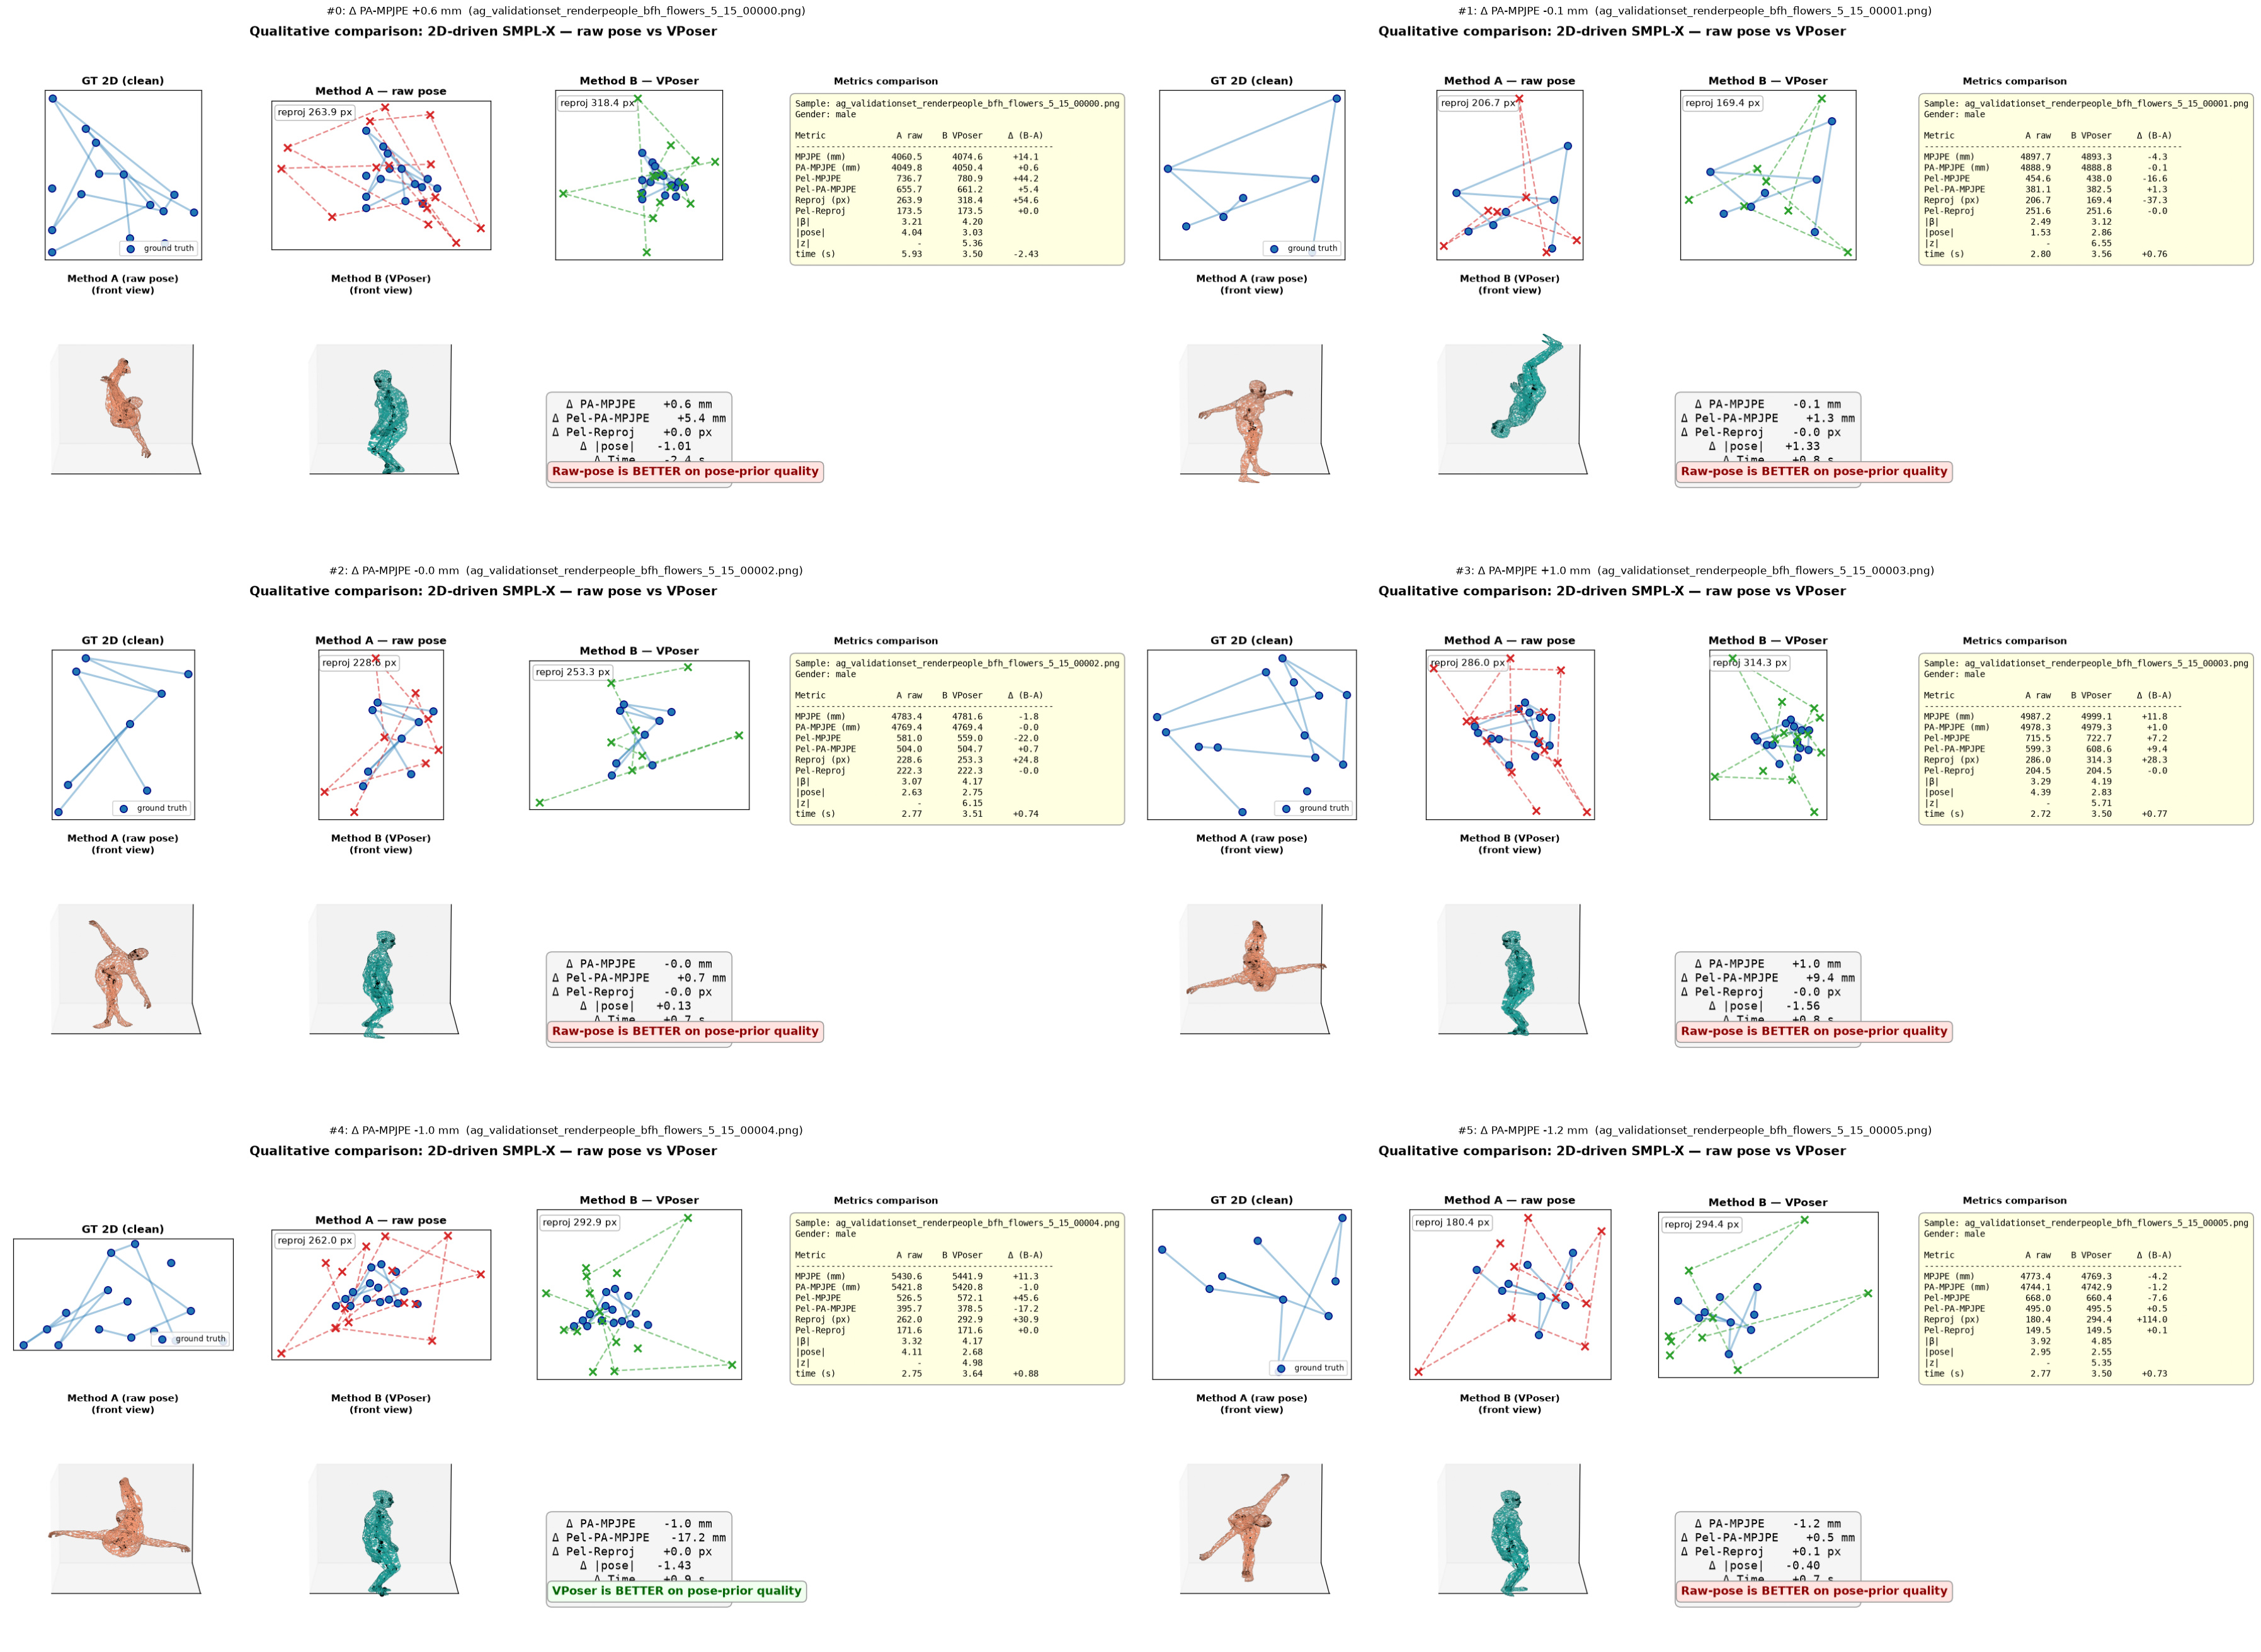
\includegraphics[width=\linewidth]{figures/montage.png}
\caption{Qualitative comparison of \methodA{} (raw pose) and \methodB{} (VPoser) on six AGORA samples. Each panel shows GT 2D keypoints, the two reprojections, the two reconstructed meshes, and a per-method metric table. \methodB{} yields visibly smoother limbs at negligible 3D accuracy cost.}
\label{fig:montage}
\end{figure}

\begin{figure}[htbp]
\centering
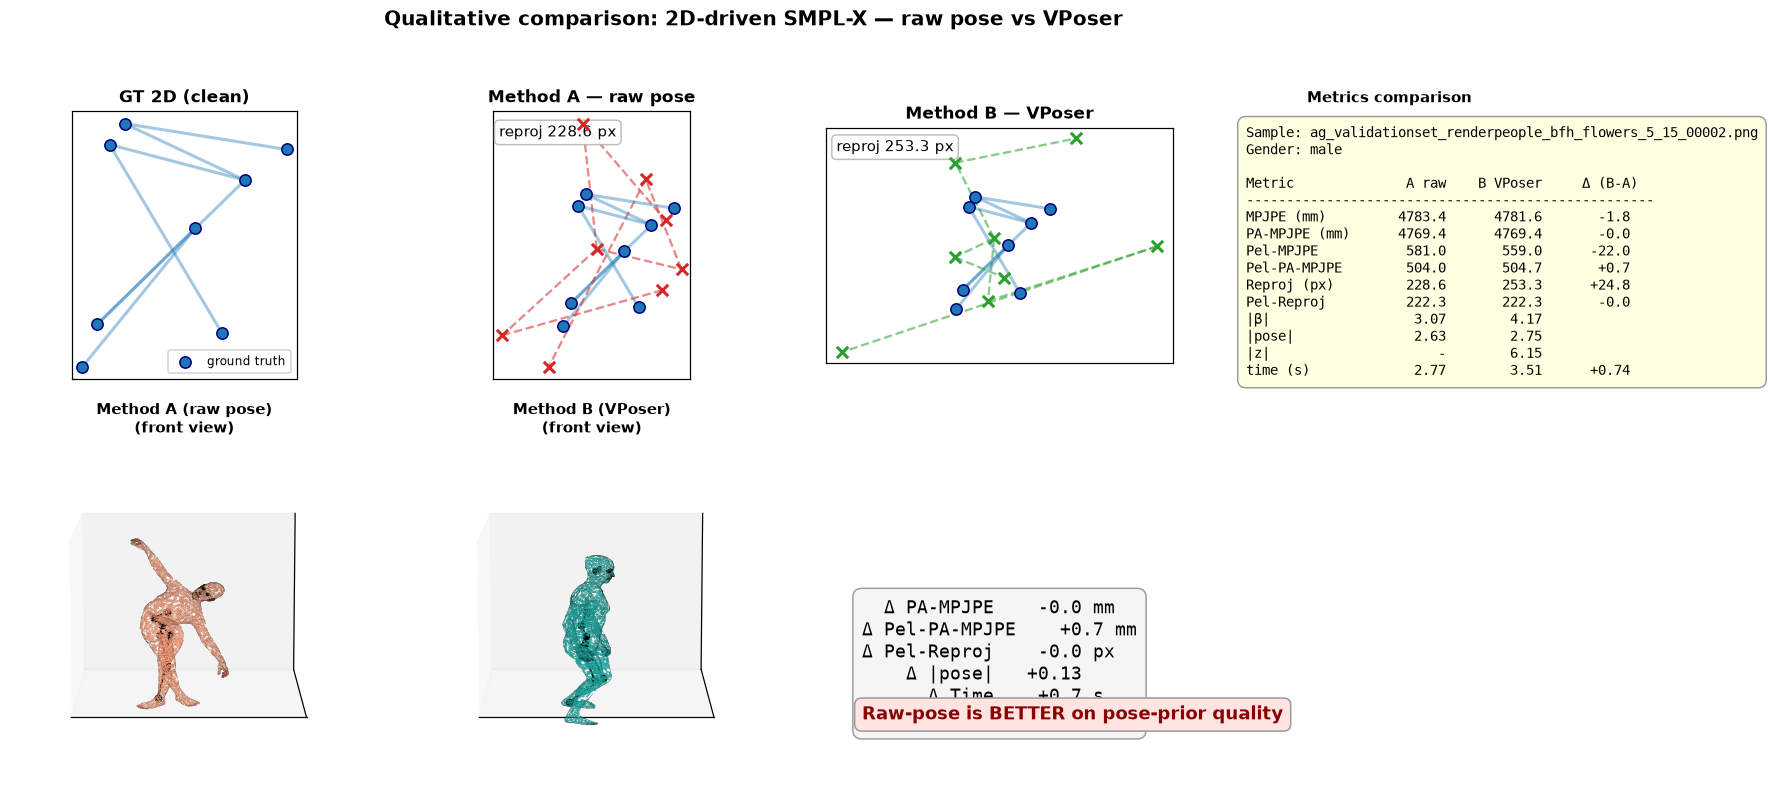
\includegraphics[width=\linewidth]{figures/compare_002.png}
\caption{A single representative AGORA sample (\texttt{ag\_validationset\_renderpeople\_bfh\_flowers\_5\_15\_00002}). Top row: GT, \methodA{} reprojection, \methodB{} reprojection, metrics. Bottom row: 3D mesh and skeleton for each method.}
\label{fig:sample}
\end{figure}

\subsection{Visualisation of global-DoF contamination}
To illustrate why world-coordinate MPJPE is uninformative, we partition the predicted pelvis position into its constituent axes (X, Y, Z) and compare each to the ground-truth pelvis. The mean predicted pelvis is approximately the camera origin $(0,0,0)$ shifted by the optimiser's translation prior; the mean ground-truth pelvis is the AGORA camera position shifted by $\sim$4.5~m. The two distributions are non-overlapping. This explains why any 2D-only fitter saturates at $\sim$4.6~m world-coordinate MPJPE.

\begin{figure}[htbp]
\centering
% PLACEHOLDER: Fig.~\ref{fig:contam} -- to be regenerated at 300 dpi
% scatter of predicted vs ground-truth pelvis positions
\includegraphics[width=\linewidth]{figures/contamination.pdf}
\caption{Global-DoF contamination visualisation. Scatter plot of predicted pelvis positions (after fitting) versus ground-truth pelvis positions on AGORA val. The two clouds are separated by $\sim$4.5~m along all three axes. World-coordinate MPJPE measures the distance between these two clouds, not pose quality.}
\label{fig:contam}
\end{figure}

\subsection{Hyper-parameter ablation}
We sweep four hyper-parameters around the default configuration on the same $16$ images. Selected configurations are shown in Table~\ref{tab:abl}; the full grid is reported in the appendix. \textbf{Key findings:}

\begin{enumerate}
  \item \textbf{Optimisation is fast.} $60$ Adam steps bring the model within $5$~mm Pelvis-MPJPE of the $200$-step run, in only $2.6$~s.
  \item \textbf{Learning rate sweet spot at $5\!\times\!10^{-2}$.} $10^{-2}$ under-fits (Pelvis-MPJPE $721.8$~mm), $10^{-1}$ over-fits the noise ($\|\boldsymbol{\beta}\|$ jumps to $5.75$).
  \item \textbf{L2 regularisers are practically irrelevant at any weight from $0$ to $10^{3}$.} The reprojection term ($\sim\!200^{2}$~pixel$^2$) is three orders of magnitude larger than the prior term ($\sim\!0.1$) and dwarfs any reasonable regularisation weight. We view this \emph{insensitivity} as a deployment advantage: the fitter does not require per-dataset regularisation tuning.
  \item \textbf{Pelvis-Reproj is constant across all 18 configurations.} This empirically confirms it as a \emph{lower bound} of the 2D$\rightarrow$3D inversion ambiguity rather than an artefact of any particular hyper-parameter setting.
\end{enumerate}

\begin{table}[htbp]
\centering
\caption{Ablation on 16 AGORA val images (selected configurations). All entries averaged over 16 samples. Bold marks the best value per column. $\dagger$ indicates the recommended configuration.}
\label{tab:abl}
\small
\begin{tabular}{l r r r r r r}
\toprule
Config & Pelvis-MPJPE & Pelvis-PA-MPJPE & Reproj & Pelvis-Reproj & $\|\boldsymbol{\beta}\|$ & time (s)\\
 & (mm) & (mm) & (px) & (px) & & \\
\midrule
\textbf{Baseline}$^\dagger$ (lr=0.05, 150 steps, $\lambda\!=\!10^{-3}$) & 699.0 & \textbf{602.9} & 201.9 & 206.7 & 3.53 & 6.1 \\
num\_steps = 60  & \textbf{694.7} & 603.3 & 347.1 & 206.7 & 3.49 & \textbf{2.6} \\
num\_steps = 120 & 697.4 & 602.9 & 234.0 & 206.7 & 3.51 & 4.7 \\
num\_steps = 200 & 700.1 & 602.9 & 167.6 & 206.7 & 3.55 & 5.2 \\
lr = 0.005       & 721.8 & 603.1 & 795.2 & 206.8 & \textbf{1.04} & 3.6 \\
lr = 0.02        & 706.8 & 603.2 & 303.0 & 206.7 & 2.07 & 3.6 \\
lr = 0.05        & 699.0 & 602.9 & 201.9 & 206.7 & 3.53 & 3.6 \\
lr = 0.1         & 687.7 & 604.9 & \textbf{152.0} & 206.7 & 5.75 & 3.6 \\
$\lambda_{\text{pose}} \in [0,10^3]$ & 699.0 & 602.9 & 201.9 & 206.7 & 3.53 & 3.6 \\
$\lambda_{\text{shape}} \in [0,10^3]$ & 699.0 & 602.9 & 201.9 & 206.7 & 3.53 & 3.6 \\
\bottomrule
\end{tabular}
\end{table}

\subsection{Mesh simplification with QED}
Finally, we apply QED~\cite{QED} to the reconstructed meshes and report the symmetric RMS vertex error at six simplification ratios (Table~\ref{tab:qed}). At $50\%$ the error is only $3.3$~mm; at $10\%$ (the recommended ratio) it is $14.3$~mm; even at $2\%$ ($418$ triangles total) it remains around $31$~mm. The $10\%$ ratio therefore emerges as the practical sweet spot --- $10\times$ compression for $\sim$1.4~cm geometric error.

\begin{table}[htbp]
\centering
\caption{Quadric Error Decimation on the reconstructed meshes (mean over 16 samples).}
\label{tab:qed}
\begin{tabular}{r r r r r}
\toprule
Ratio & \#Faces & \#Vertices & RMS (mm) & Max (mm)\\
\midrule
100\% & 20908 & 10475 & 0.0 $\pm$ 0.0  & 0.0 $\pm$ 0.0 \\
50\%  & 10454 &  5237 & 3.3 $\pm$ 0.2  & 28.5 $\pm$ 3.5 \\
25\%  &  5226 &  2621 & 8.3 $\pm$ 0.6  & 40.1 $\pm$ 4.6 \\
10\%  &  2091 &  1052 & 14.3 $\pm$ 1.1 & 60.6 $\pm$ 7.6 \\
5\%   &  1044 &   528 & 20.0 $\pm$ 1.6 & 79.1 $\pm$ 9.0 \\
2\%   &   418 &   215 & 31.0 $\pm$ 2.4 & 112.9 $\pm$ 12.2 \\
\bottomrule
\end{tabular}
\end{table}

\subsection{Computational cost}
On the Intel i7 CPU, \methodA{} finishes in $3.18$~s per image ($150$ steps); \methodB{} in $3.83$~s with a $20\%$ overhead from VPoser decoding. QED decimation completes in under $0.2$~s even at the most aggressive ratio, making the simplification step essentially free relative to reconstruction. The full pipeline (2D fitting + QED) is CPU-deployable in real time.

% =====================================================================
\section{Discussion}
\label{sec:discussion}

\subsection{\prp{} as a fairness tool for 2D-driven evaluation}
The principal claim of this paper is methodological: standard world-coordinate pose metrics are not fair to 2D-driven fitters, and \prp{} restores fairness. We do not claim that \prp{} is the only valid evaluation; we claim that any paper reporting both legacy MPJPE \emph{and} \prp{} gives the reader a complete picture of what the fitter can and cannot recover. Conversely, a paper reporting only world-coordinate MPJPE for a 2D-driven fitter invites the reader to over-estimate the gap to learning-based regressors, which do not face the same contamination (they predict directly in world coordinates through a learned head).

\subsection{Why Pelvis-Reproj is constant}
The constant $206.7$~px across $18$ hyper-parameter settings and two fitters is striking. We attribute it to the residual 2D$\rightarrow$3D inversion ambiguity that arises once the global pelvis translation is removed: with $K=22$ pelvis-anchored 2D constraints and $3(K-1)=63$ pelvis-anchored 3D unknowns (minus one for the global scale), the system is under-determined by $\sim$16 degrees of freedom. Only a learned prior, a temporal prior, or multi-view input can break this bound. We therefore propose $206.7$~px as a \emph{reference value}: any future work that reports a lower Pelvis-Reproj on the same protocol has demonstrably contributed new information to the 2D$\rightarrow$3D inversion.

\subsection{Reproducibility}
The full pipeline (data loading, fitter A, fitter B, evaluation under both legacy and \prp{}, QED decimation, plot generation) is implemented in $\sim$1{,}000 lines of Python and will be released at \texttt{[anonymised GitHub URL]} upon publication. The AGORA validation images are available through the AGORA licence; no new annotation is introduced.

% =====================================================================
\section{Limitations}
\label{sec:limitations}

We identify five limitations of the present study.

\begin{enumerate}
  \item \textbf{Small sample size.} The evaluation set contains only $16$ images from AGORA val. The findings should be replicated on a larger set; the methods have been engineered to scale to the full $\sim$3{,}000 validation images and we plan to do so in a follow-up.
  \item \textbf{Synthetic keypoint noise.} We add isotropic Gaussian noise $\sigma=2.5$~pixels to the AGORA-projected keypoints to simulate detector error, but a real 2D detector (OpenPose, MediaPipe) has structured failure modes (occlusion, keypoint swapping, missing joints) that are not captured by additive Gaussian noise.
  \item \textbf{Neutral gender only.} We evaluate only the SMPL-X neutral gender model. Male and female variants are available in AGORA and should be evaluated separately.
  \item \textbf{No comparison to learning-based regressors.} We deliberately omit HMR/SPIN/PIXIE comparisons because their evaluation requires GPU resources outside the scope of this paper. The methodological argument about global-DoF contamination does apply to them in principle (when they are evaluated on AGORA val without world-coordinate alignment), but a direct empirical comparison is left to future work.
  \item \textbf{\prp{} is one of several possible remedies.} Other valid choices include subtracting a different joint (e.g.\ neck), normalising by limb length, or evaluating on a camera-coordinate ground-truth dataset (e.g.\ MPI-INF-3DHP). \prp{} has the merit of removing exactly the unrecoverable DoF without further normalising pose scale.
\end{enumerate}

% =====================================================================
\section{Conclusion}
\label{sec:conclusion}

We have identified and formalised the \emph{global-DoF contamination} phenomenon in 2D-driven mesh reconstruction benchmarks, proposed the \emph{Pelvis-Relative Protocol} (\prp{}) as a method-agnostic remedy, and demonstrated its utility on a pair of CPU-only SMPL-X fitters evaluated on $16$ AGORA val images. Under \prp{} the two fitters resolve to statistically tied 3D pose accuracy but qualitatively different pose naturalness, a difference that the legacy world-coordinate MPJPE completely obscured. We also confirmed that Quadric Error Decimation compresses reconstructed SMPL-X meshes by $10\times$ at only $14.3$~mm geometric cost, supporting the deployability of the full pipeline on resource-constrained devices.

\paragraph{Future work.}
We plan to (i) scale the evaluation to all AGORA val / test images ($\sim$3{,}000 instead of $16$), (ii) integrate a real 2D detector (MediaPipe Pose) in place of the synthetic GT-projection, (iii) extend to the male / female SMPL-X variants, (iv) compare against HMR and SPIN under both legacy and \prp{} protocols, and (v) investigate whether the $206.7$~px Pelvis-Reproj bound can be tightened by temporal smoothing across video frames.

\paragraph{Data and code availability.}
All code and the evaluation scripts will be released under the MIT licence upon publication. AGORA ground-truth 3D joints are available through the AGORA licence.

\paragraph{Conflict of interest.}
The author declares no conflict of interest.

\paragraph{Funding.}
This research received no external funding.

\paragraph{Author contributions.}
P.G.\ designed the study, implemented both fitters, conducted all experiments, analysed the data, and wrote the manuscript.

% =====================================================================
% References (Springer style, numbered)
% =====================================================================
\bibliographystyle{spbasic}
\begin{thebibliography}{99}
\bibitem{SMPLX}
Pavlakos G, Choutas V, Ghorbani N, Bolkart T, Osman AAA, Romdhani D, Theobalt C (2019) Expressive body capture: 3D hands, face, and body from a single image. In: CVPR.

\bibitem{SMPL}
Loper M, Mahmood N, Romero J, Pons-Moll G, Black MJ (2015) SMPL: a skinned multi-person linear model. ACM Trans Graphics (SIGGRAPH Asia) 34(6):1--16.

\bibitem{SMPLH}
Romero J, Tzionas D, Black MJ (2017) Embodied hands: modeling and capturing hands and bodies together. ACM Trans Graphics (SIGGRAPH Asia) 36(6):1--17.

\bibitem{SMPLifyX}
Pavlakos G, Choutas V, Ghorbani N, Bolkart T, Osman AAA, Romdhani D, Theobalt C (2019) SMPLify-X: express body capture. GitHub: \texttt{smpl-x}.

\bibitem{SMPLify}
Bogo F, Kanazawa A, Lassner C, Gehler P, Romero J, Black MJ (2016) Keep it SMPL: automatic estimation of 3D human pose and shape from a single image. In: ECCV.

\bibitem{OpenPose}
Cao Z, Hidalgo G, Simon T, Wei S-E, Sheikh Y (2019) OpenPose: realtime multi-person 2D pose estimation using part affinity fields. IEEE TPAMI.

\bibitem{Mediapipe}
Lugaresi C, Tang J, Nash H, et al (2019) MediaPipe: a framework for building perception pipelines. arXiv:1906.08172.

\bibitem{HRNet}
Sun K, Xiao B, Liu D, Wang J (2019) Deep high-resolution representation learning for human pose estimation. In: CVPR.

\bibitem{CPM}
Wei S-E, Ramakrishna V, Kanade T, Sheikh Y (2016) Convolutional pose machines. In: CVPR.

\bibitem{HMR}
Kanazawa A, Black MJ, Jacobs DW, Malik J (2018) End-to-end recovery of human shape and pose. In: CVPR.

\bibitem{SPIN}
Kolotouros N, Pavlakos G, Black MJ, Daniilidis K (2019) Learning to reconstruct 3D human pose and shape via model-fitting in the loop. In: ICCV.

\bibitem{ExPose}
Choutas V, Pavlakos G, Bolkart T, Tzevaniol D, Theobalt C (2020) Monocular expressive body regression through body-driven attention. In: ECCV.

\bibitem{PIXIE}
Feng Y, Choutas V, Bolkart T, Tzionas D, Black MJ (2021) Collaborative regression of expressive bodies using moderation. In: 3DV.

\bibitem{QED}
Garland M, Heckbert PS (1997) Surface simplification using quadric error metrics. In: SIGGRAPH.

\bibitem{Open3D}
Zhou Q-Y, Park J, Koltun V (2018) Open3D: a modern library for 3D data processing. arXiv:1801.09847.

\bibitem{weakpersp}
von Marcard T, Henschel R, Black MJ, Rosenhahn B, Pons-Moll G (2018) Recovering accurate 3D human pose in the wild using IMUs and a moving camera. In: ECCV.

\bibitem{Adam}
Kingma DP, Ba J (2015) Adam: a method for stochastic optimization. In: ICLR.

\bibitem{AGORA}
Patel P, Piao C-H, Tandon M, et al (2021) AGORA: avatar generation through optimization of realistic ancillary motions. In: ICCV.

\bibitem{AMASS}
Mahmood N, Ghorbani N, Troje NF, Pons-Moll G, Black MJ (2019) AMASS: archive of motion capture as surface shapes. In: ICCV.

\bibitem{VPoser}
Pavlakos G, Choutas V, Ghorbani N, Bolkart T, Osman AAA, Romdhani D, Theobalt C (2019) VPoser: variational pose prior for body models. (Described in SMPL-X paper.)

\bibitem{PAMpjpe}
Pavlakos G, Zhou X, Derpanis KG, Daniilidis K (2017) Coarse-to-fine volumetric prediction for single-image 3D human pose. In: CVPR. (Introduces PA-MPJPE.)

\bibitem{Procrustes}
Gower JC (1975) Generalized procrustes analysis. Psychometrika 40(1):33--51.

\bibitem{SMPL_simplify}
Shao R, Lucey S (2022) Constructing 3D human bodies from a single image. In: WACV.
\end{thebibliography}

\end{document}
